

Dislocations are line defects in crystals that are important, amongst other reasons, because they are responsible for plastic deformation. Though the character of dislocations varies in a continuous fashion there are two limiting cases: Edge dislocations can be introduced to a perfect crystal by the introduction of an extra half plane of atoms, the termination of this half plane is the dislocation, see \autoref{fig:Edge_disloc_loop}. Screw dislocations are formed by shearing a region of crystal such that the lattice planes form a helix, the centre of the helix is then the dislocation, this is shown in \autoref{fig:screw_disloc}. Mixed dislocations have some of the character of both these end members.



\begin{figure}
\centering

\begin{subfigure}{0.4\textwidth}
\centering
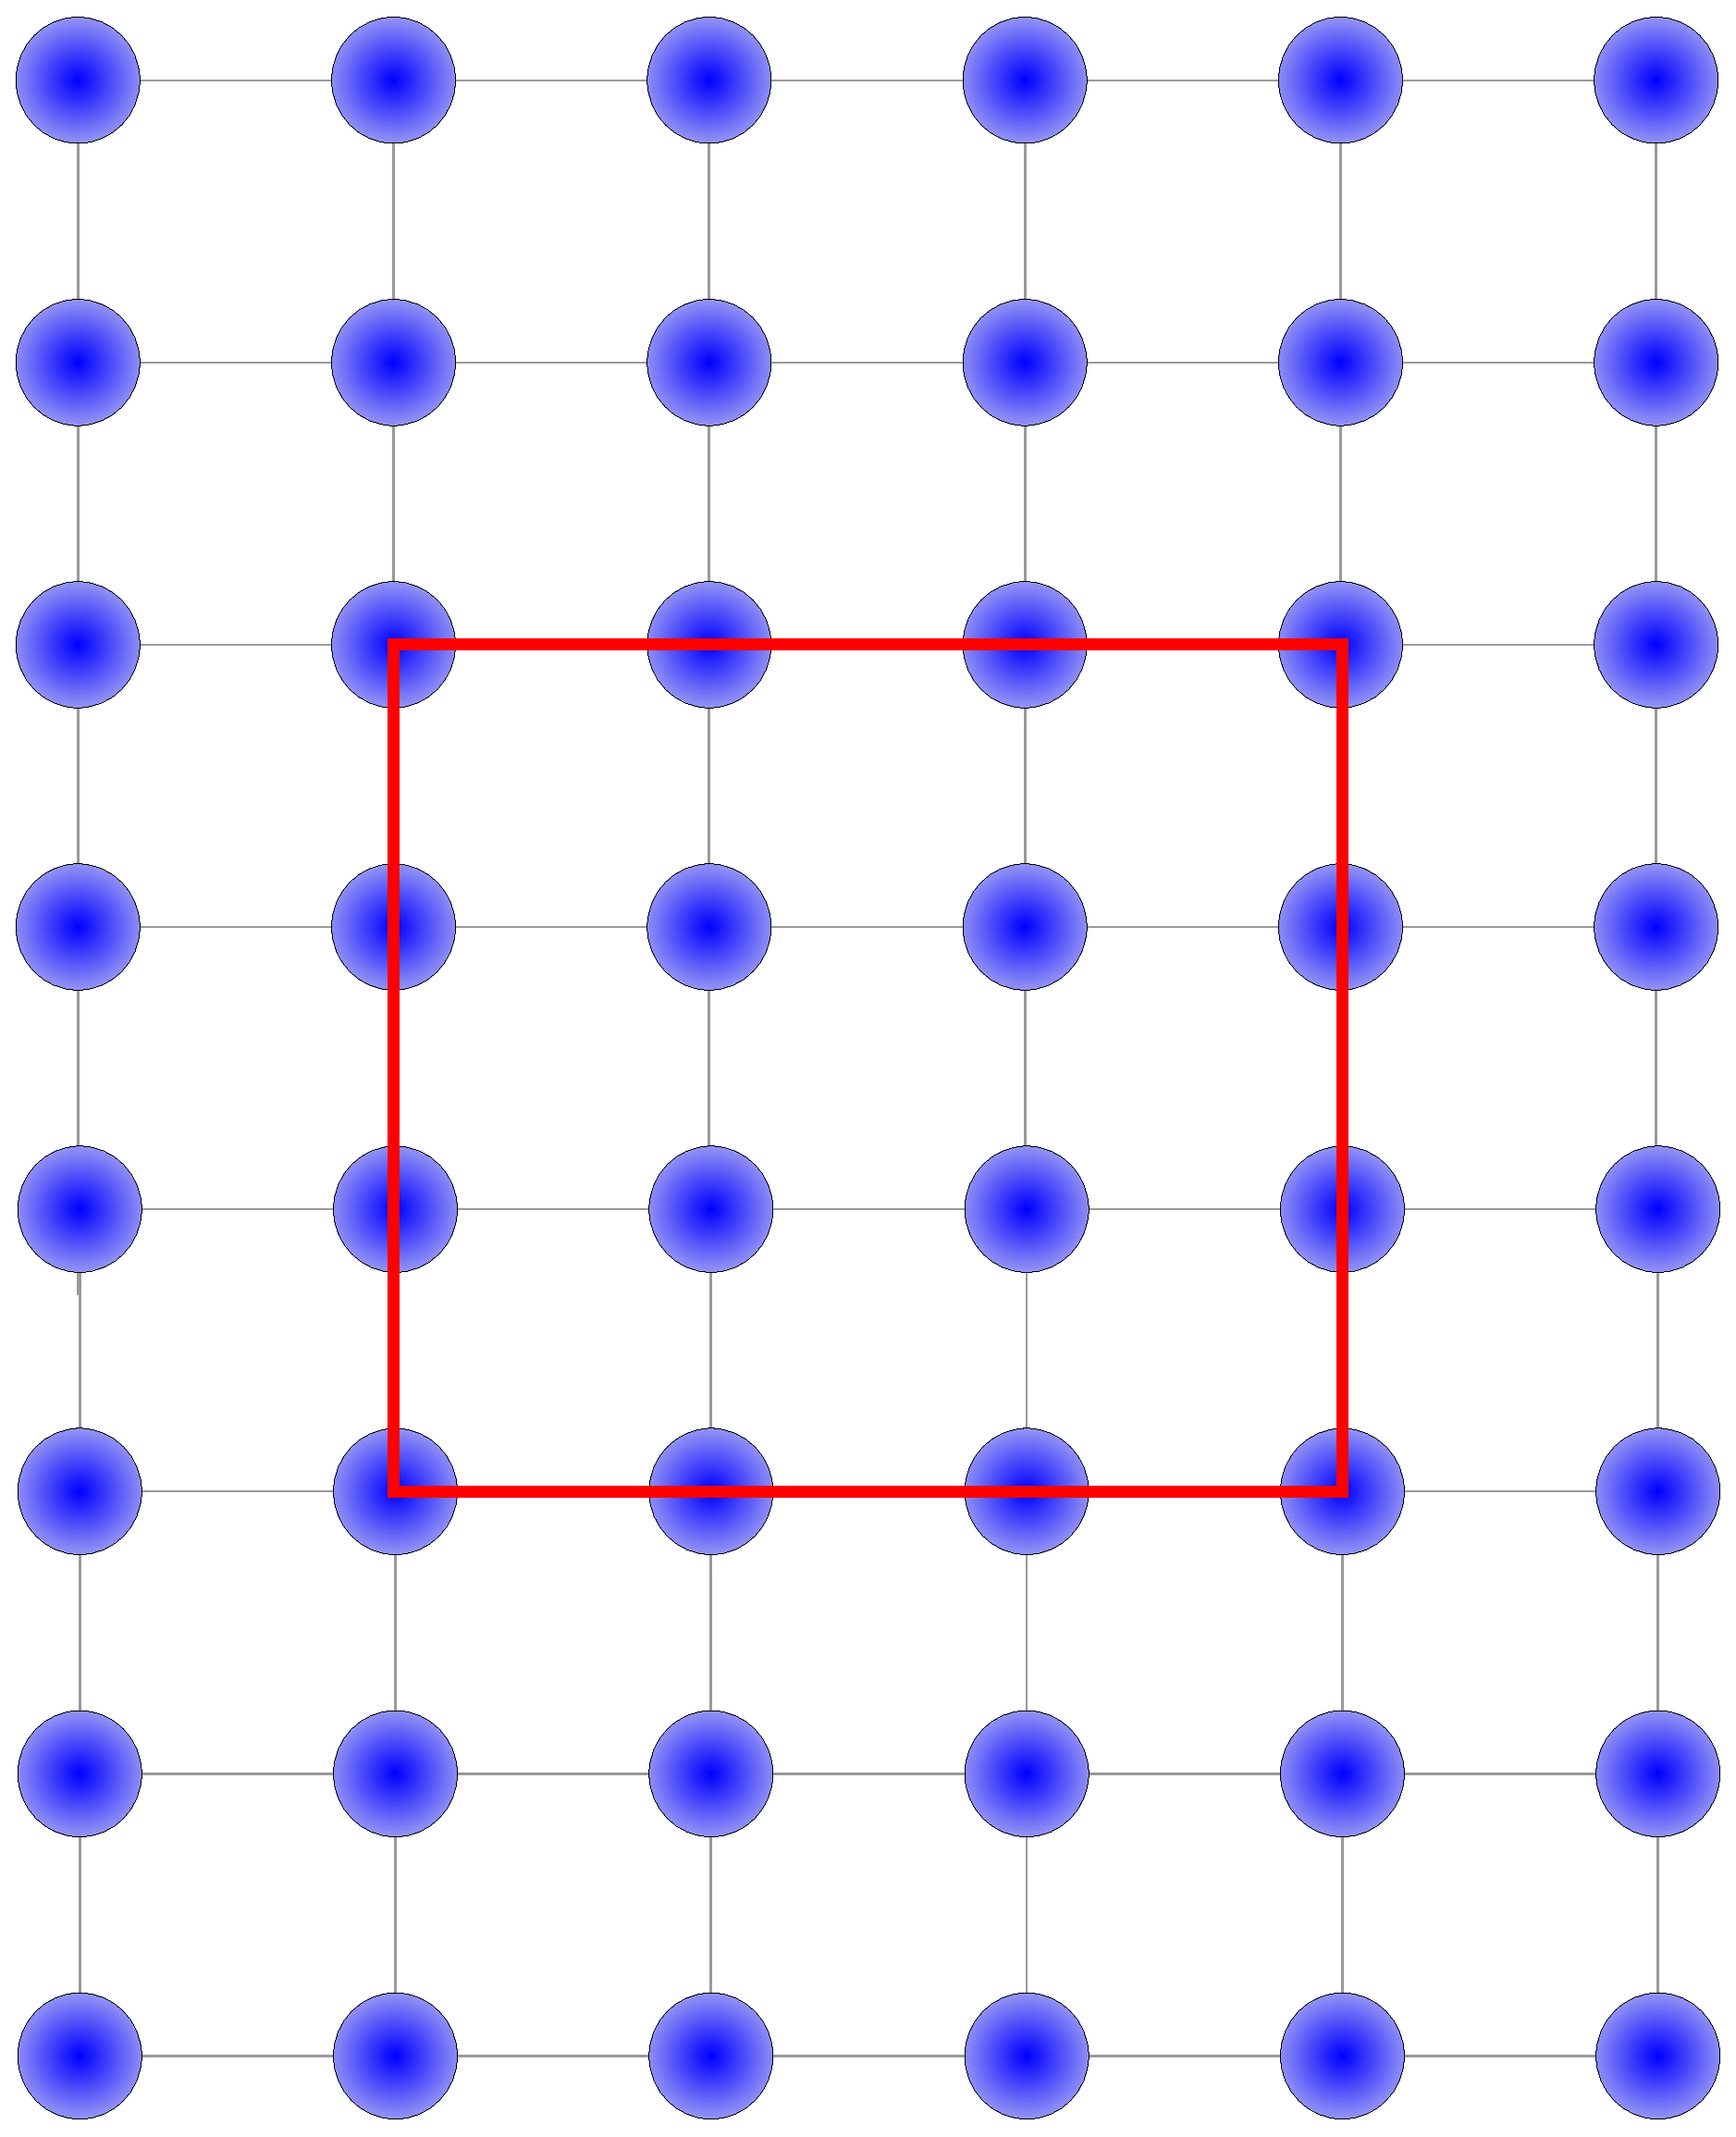
\includegraphics[height=2.5in]{Perfect_crystal_loop}
\caption{A perfect crystal with a complete circuit shown in red.}
\end{subfigure}
\begin{subfigure}{0.4\textwidth}
\centering
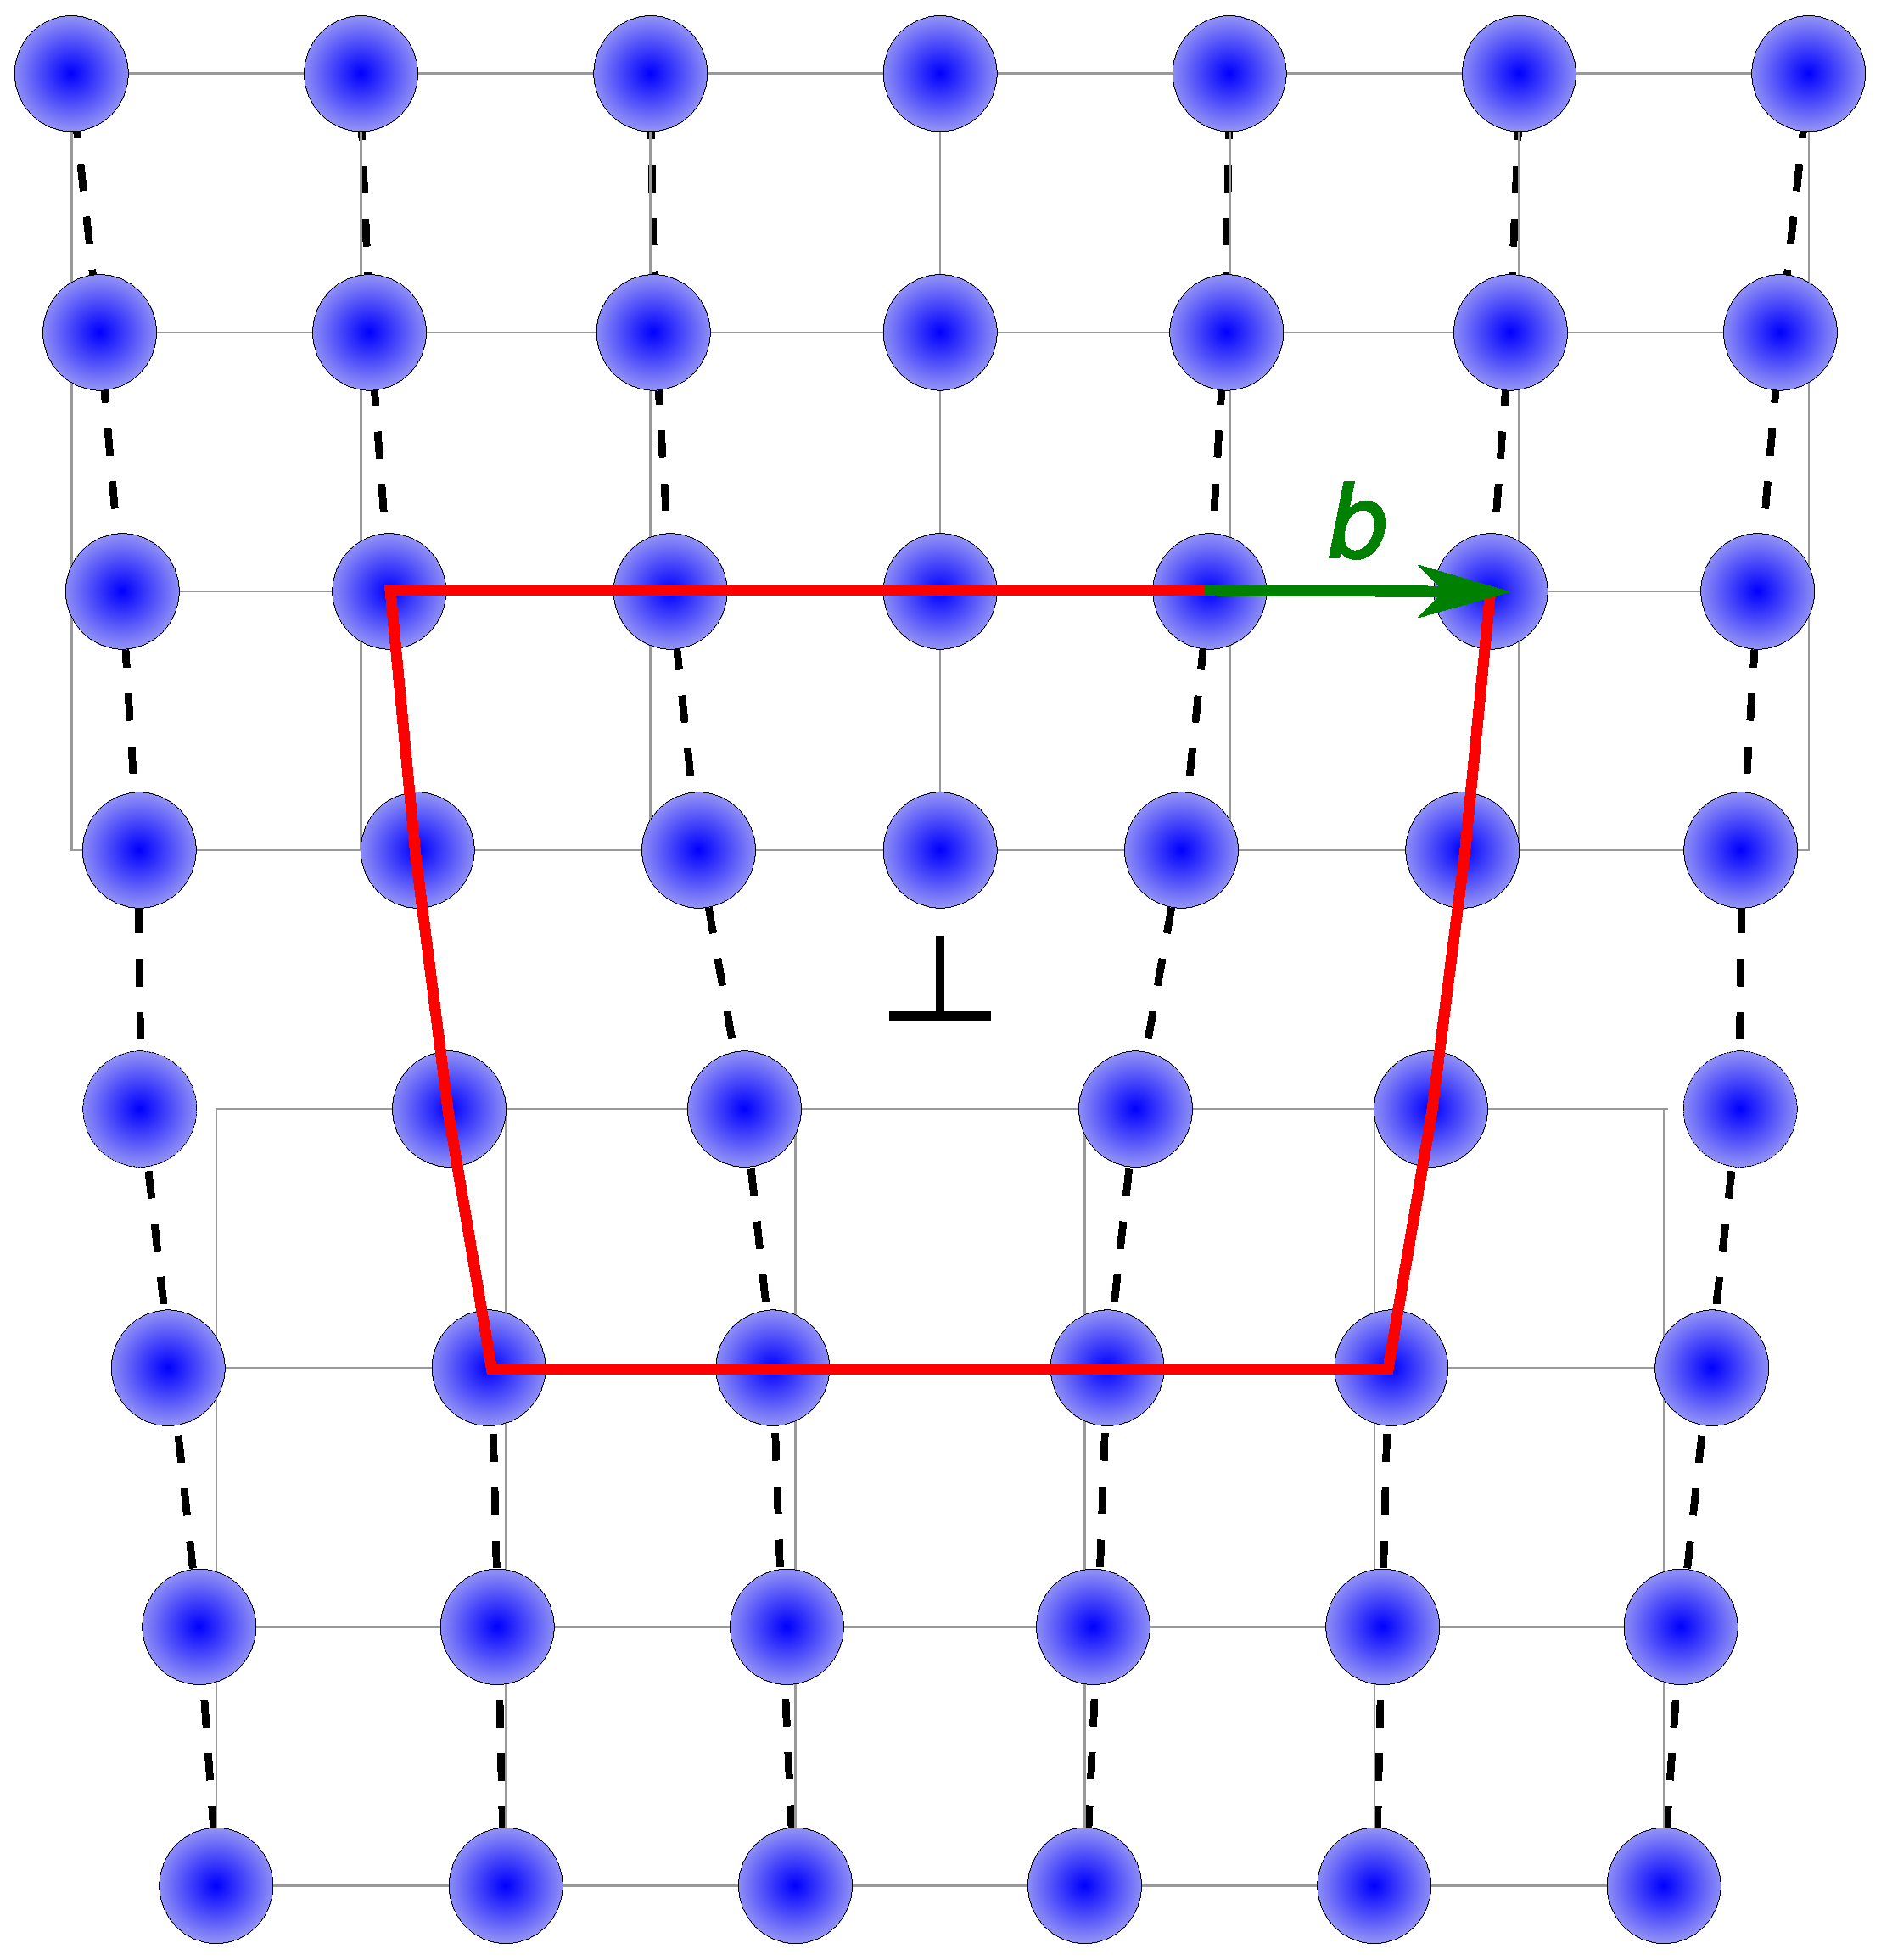
\includegraphics[height=2.5in]{Edge_Dislocation_loop}
\caption{An edge dislocation with an incomplete circuit. \label{fig:Edge_disloc_loop}}
\end{subfigure}

\caption[A Burgers loop around an edge dislocation.]{Inserting a half plane of atoms which terminate in a dislocation and a Burgers circuit to show the Burgers vector. \label{fig:burgers_loops}}

\end{figure}

\begin{figure}
\centering
\captionsetup{width=0.8\textwidth,font={sf,scriptsize},labelfont=bf}
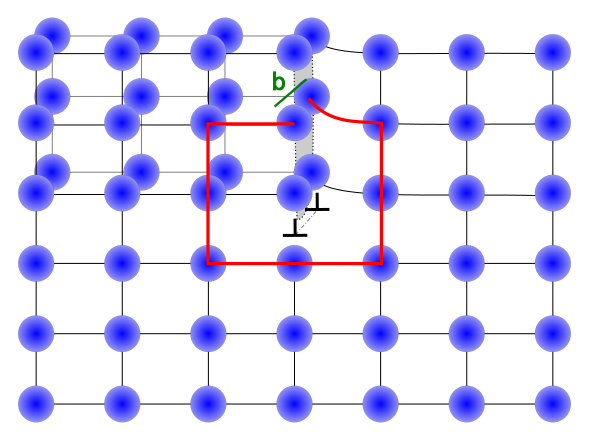
\includegraphics[width=0.7\textwidth]{screw_disloc_loop}
\caption[A Burgers loop around a screw dislocation.]{Schematic of a screw dislocation with a Burgers loop formed in a similar way to \autoref{fig:burgers_loops}. The displacement is parallel to the dislocation line in contrast with edge dislocations. The atomic positions are schematic only, the displacements being concentrated unphysically into one half plane. \label{fig:screw_disloc}}
\end{figure}




Dislocations can be described in terms of a slip direction, a line direction and a slip plane. The slip direction is simply the direction parallel to the Burgers vector, this is the relative displacement caused by the passage of a dislocation through a region of crystal. The identification of the Burgers vector is done with a Burgers loop, comprised of steps between nearest neighbours that would form a closed in a perfect crystal. The same set of steps is undertaken in a dislocated crystal and the loop is no longer closed; the displacement vector between the endpoints of the open loop is the Burgers vector. This is shown for an edge dislocation in \autoref{fig:burgers_loops}, where the Burgers vector is perpendicular to the line vector, and a screw dislocation in \autoref{fig:screw_disloc}, where the Burgers vector is parallel to the line vector. The line direction can and does vary along the length of the dislocation but is simply the line defined by the defective region of crystal. 

The slip plane is the crystallographic plane in which the dislocation can move and must contain the slip direction and line direction. Where the line and the slip directions are not parallel the slip plane is defined by these two vectors, but for screw dislocations, for which the slip direction and the line direction are parallel, the plane is not constrained. Thus screw dislocations can to change the plane over which they are move; this process is known as cross slip \cite{Hirth_Lothe1982intro}.

Real dislocations are not neat and instead of lining up with convenient crystallographic axes will curve and bend. This usually gives rise to a mixed character and are usually described as the sum of edge and screw components.

There are conventions about the sense of dislocations; if the line vector is taken to be into the page and the sense of the Burgers loop is right handed then the Burgers vector is defined from the start to the finish of the Burgers loop. Given that the symmetry of most of the crystals of interest is high, these choices are arbitrary. One useful consequence of this description is that if sense of a dislocation is reversed then its stress/strain field will also reverse in sign. Hence oppositely signed dislocations attract to lower the stored elastic energy and potentially to annihilate line length, while like-signed dislocations will repel to lower the elastic stored energy.



\FloatBarrier

\subsection{Historical overview}


In the early twentieth century there were many observations of real world materials strengths that could not be reconciled with the theoretical shearing strength of a perfect plane of atoms. For a long time this was neglected because, as \citet{gordon1991} explains ``until about 1934 the Establishment explanation of these phenomena was remarkably unconvincing and seems to have reflected mainly a desire not to be asked embarrassing questions.''

In 1934 the edge dislocation was proposed by \citet{orowan1934i,Orowan1934ii,Orowan1934iii}, \citet{Taylor1934}, and \citet{polanyi1934} to explain the discrepancy between the ideal strength of crystal and the observed strengths of real materials. It was around this time that work undertaken by \citet{Volterra1907} and others, particularly \citet{love1920},
on elastic behaviour of homogeneous isotropic continua was related to plastic flow of crystalline materials; idealised dislocations in elastic continua are termed \emph{Volterra dislocations}. By the end of the decade \citet{burgers1939} had described screw dislocations. 

It was not until the 1950s that experimental evidence for the existence of dislocations was produced; the initial evidence was growth surfaces of single crystals, preferential etching of a crystalline material at dislocations and x-ray studies of arrays of dislocations in the bulk \cite{Forty1954}. 

\citet{Frank1949} predicted, in 1949, that a step could terminate by the intersection of a dislocation with a free surface, or conversely a dislocation intersecting with a free surface would necessarily create a step; these were observed soon after in 1950 by \citet{Griffin1950}. Preferential etching of dislocations was observed by \citet{horn1952holes} who matched the configuration of etch pits with the pre-existing surface growth features that arise from screw dislocations. The effect of plastic work and subsequent recovery on Laue spots (the xray beams diffracted by a single crystal) provide evidence of arrays of dislocations. The process was described by \citet{Cottrell1949}: Initially sharp Laue spots exist in a perfect crystal. Plastic work smears the spots by introducing a homogeneous distribution of dislocations and the spots then split into distinct sharp spots during recovery as dislocations align into arrays that form sub-grains with small misalignments across the new low angle grain boundaries.


An edge dislocation was first imaged in 1956 by \citet{Menter1956} in platinum phthalocyanine. The large organic complex with a platinum atom at the centre produces widely spaced rows of platinum atoms suitable for imaging with transmission electron microscopy.




\subsection{The stress required to move a dislocation}



Though mathematical descriptions of dislocations in isotropic elastic continua date back to 1907 \cite{Volterra1907} the energies and forces around dislocations in crystalline lattices were not considered until later. In 1940 \citet{Dehlinger1940} and \citet{Peierls1940} presented dislocation models. The former presented the application of the Frenkel-Kontorova model, a one dimensional array of balls connected by springs on a periodic potential/substrate, to approximate a dislocation.

The latter, Rudolph Peierls, working during the advent of quantum mechanics presented the first formal solution for the energy changes as a dislocation moves in a rather short note \cite{Peierls1940} and the idea was later extended by \citet{Nabarro1947}. The model is remarkably simple; consider two semi-infinite perfect crystals with their lattices aligned but with some initial offset between them as shown in \autoref{fig:semi_infinite_crystals}. We can join them along what will become the slip plane. An edge dislocation is formed where the energy of the system is lowered by displacing atoms from their initial positions to localise the misalignments around the dislocation core, usually taken to be the origin. i.e. when the energy of a planar defect is higher than that of the linear defect and dislocation will form.



\begin{figure}
\centering

    \begin{subfigure}{0.4\textwidth}
        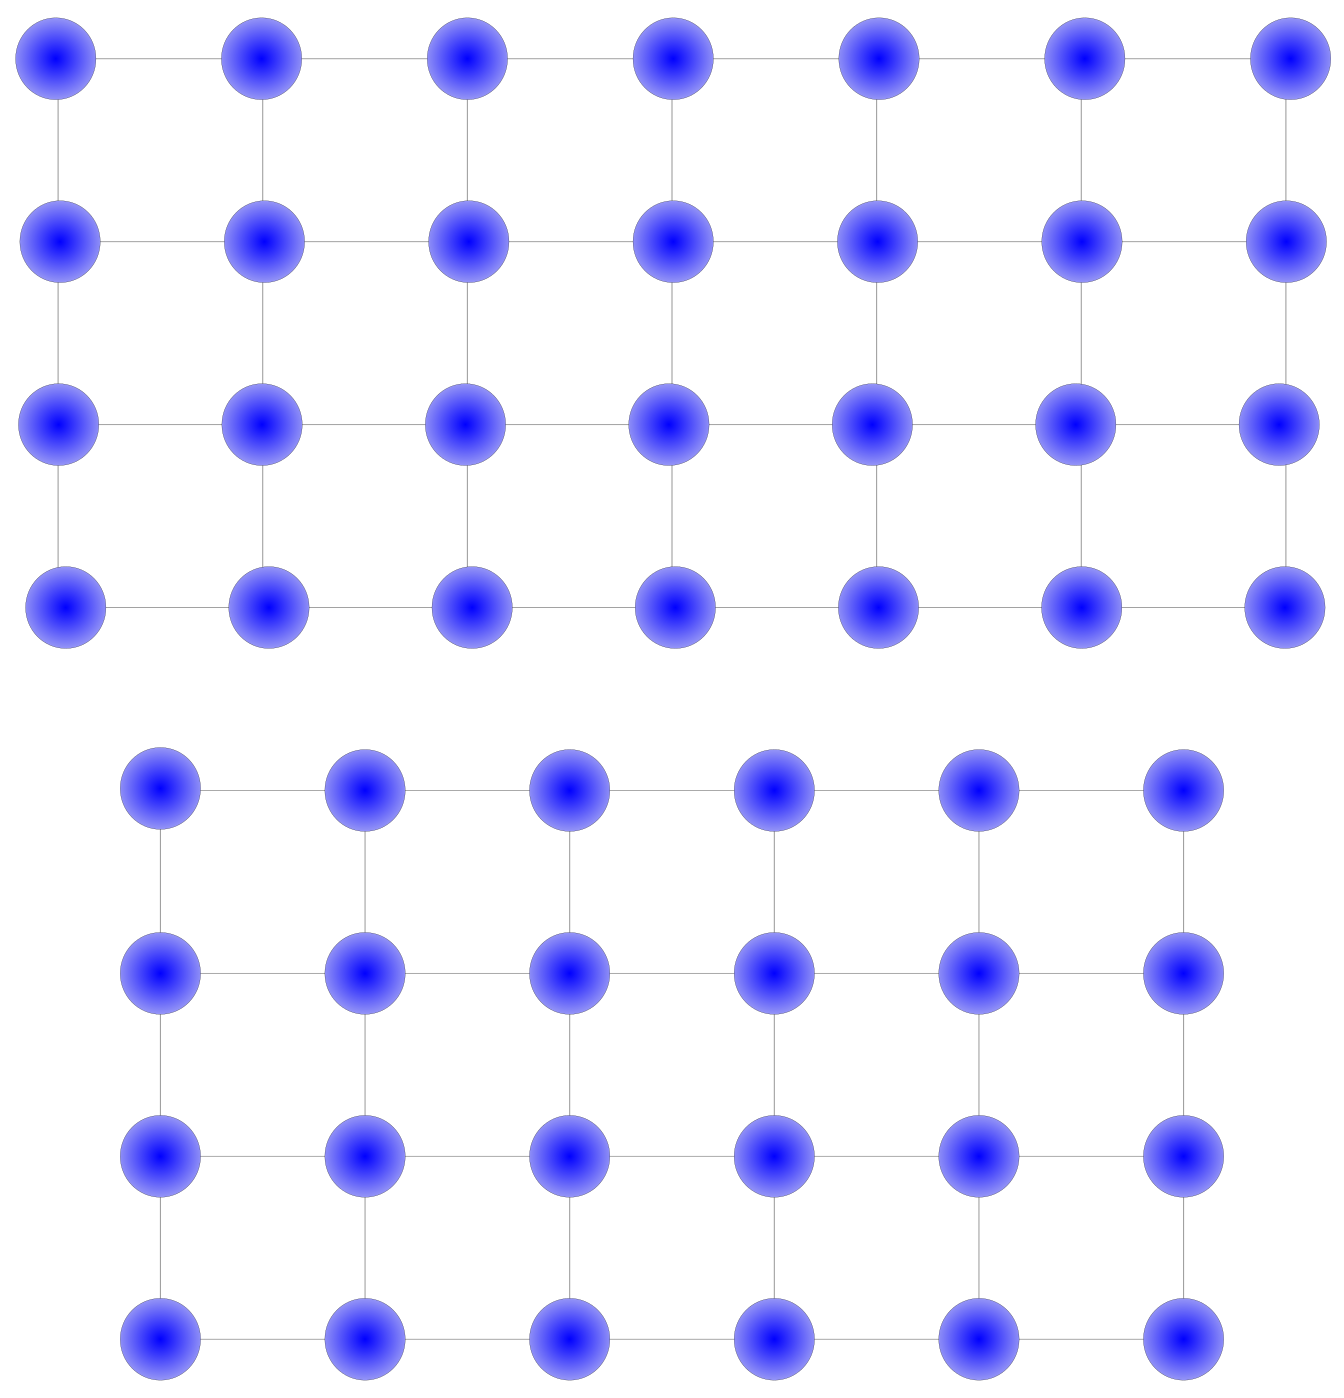
\includegraphics[width=\textwidth]{Half_crystals}
        \caption{Two semi-infinite crystals \label{fig:semi_infinite_crystals}}
    \end{subfigure}
    
    \vspace{0.5cm}
    
    \begin{subfigure}{0.4\textwidth}
        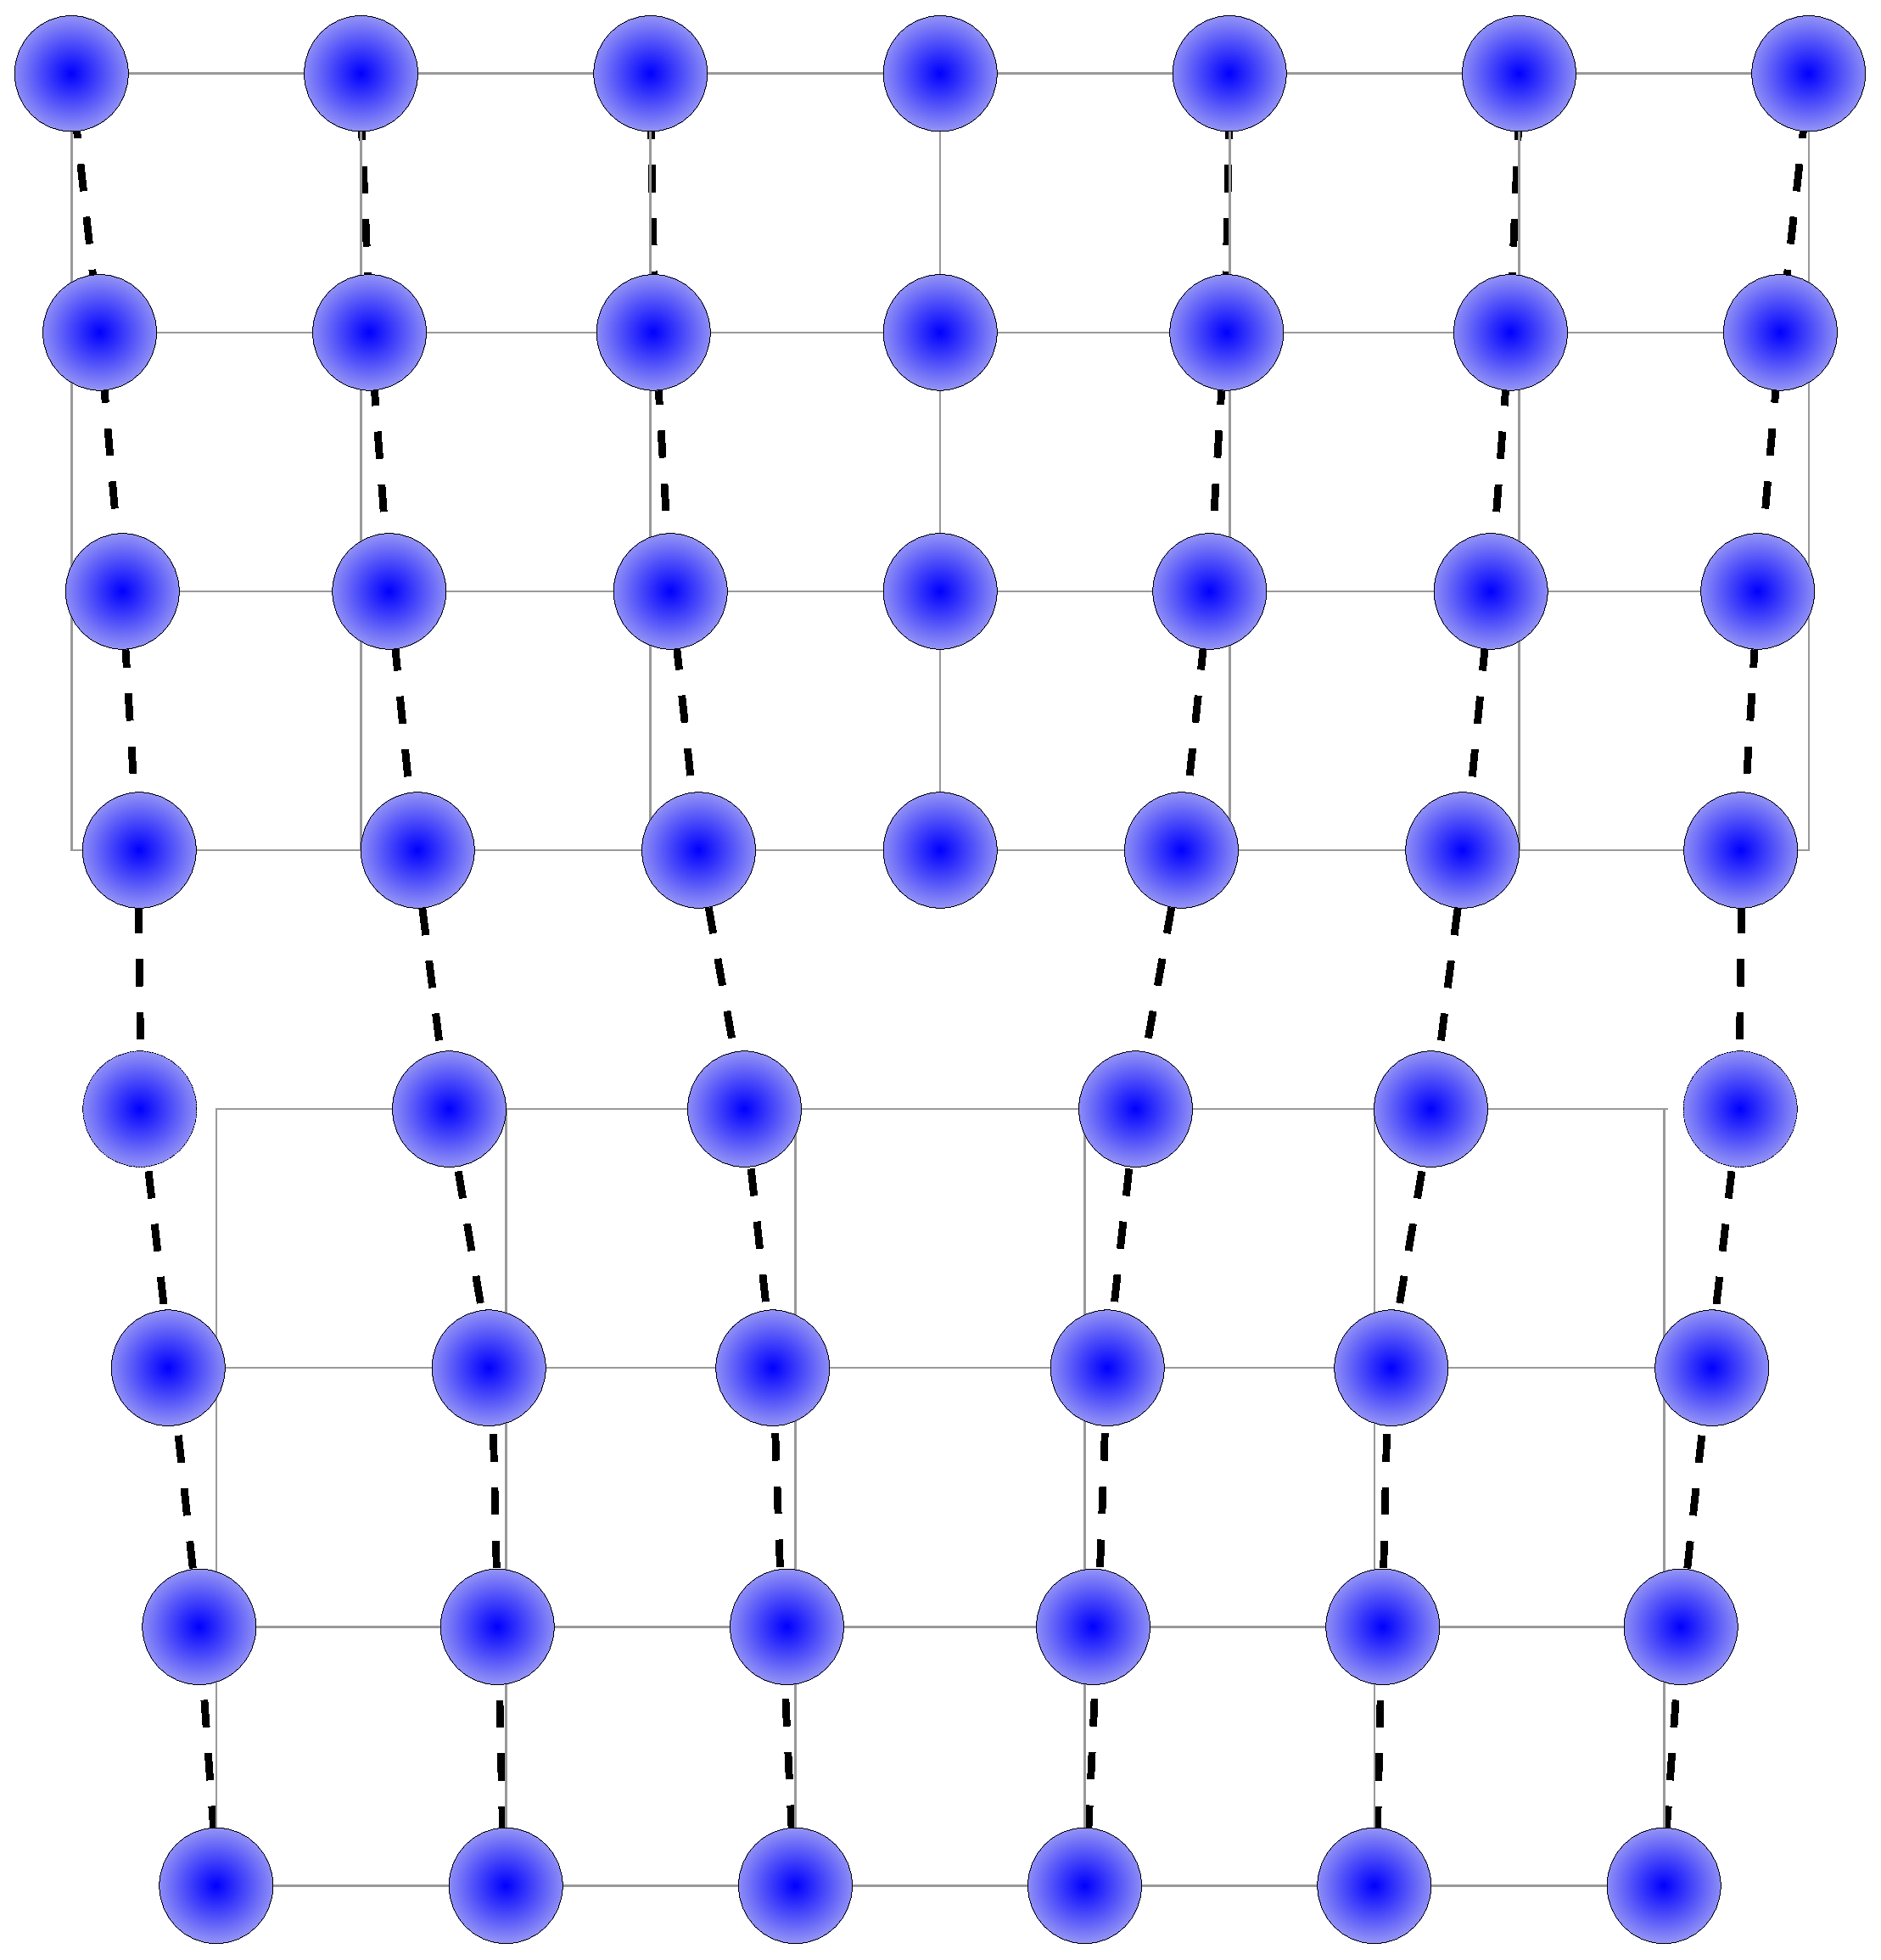
\includegraphics[width=\textwidth]{Edge_Dislocation}
        \caption{A schematic edge dislocation\label{fig:joined_half_crystals}}
    \end{subfigure}

    \captionsetup{width=0.5\textwidth}
    \caption[Building an edge dislocation.]{Schematics showing the creation of an edge dislocation in a simple square lattice by the joining of two misaligned half crystals. \label{fig:edge_disloc}}
\end{figure}

\begin{figure}
\centering
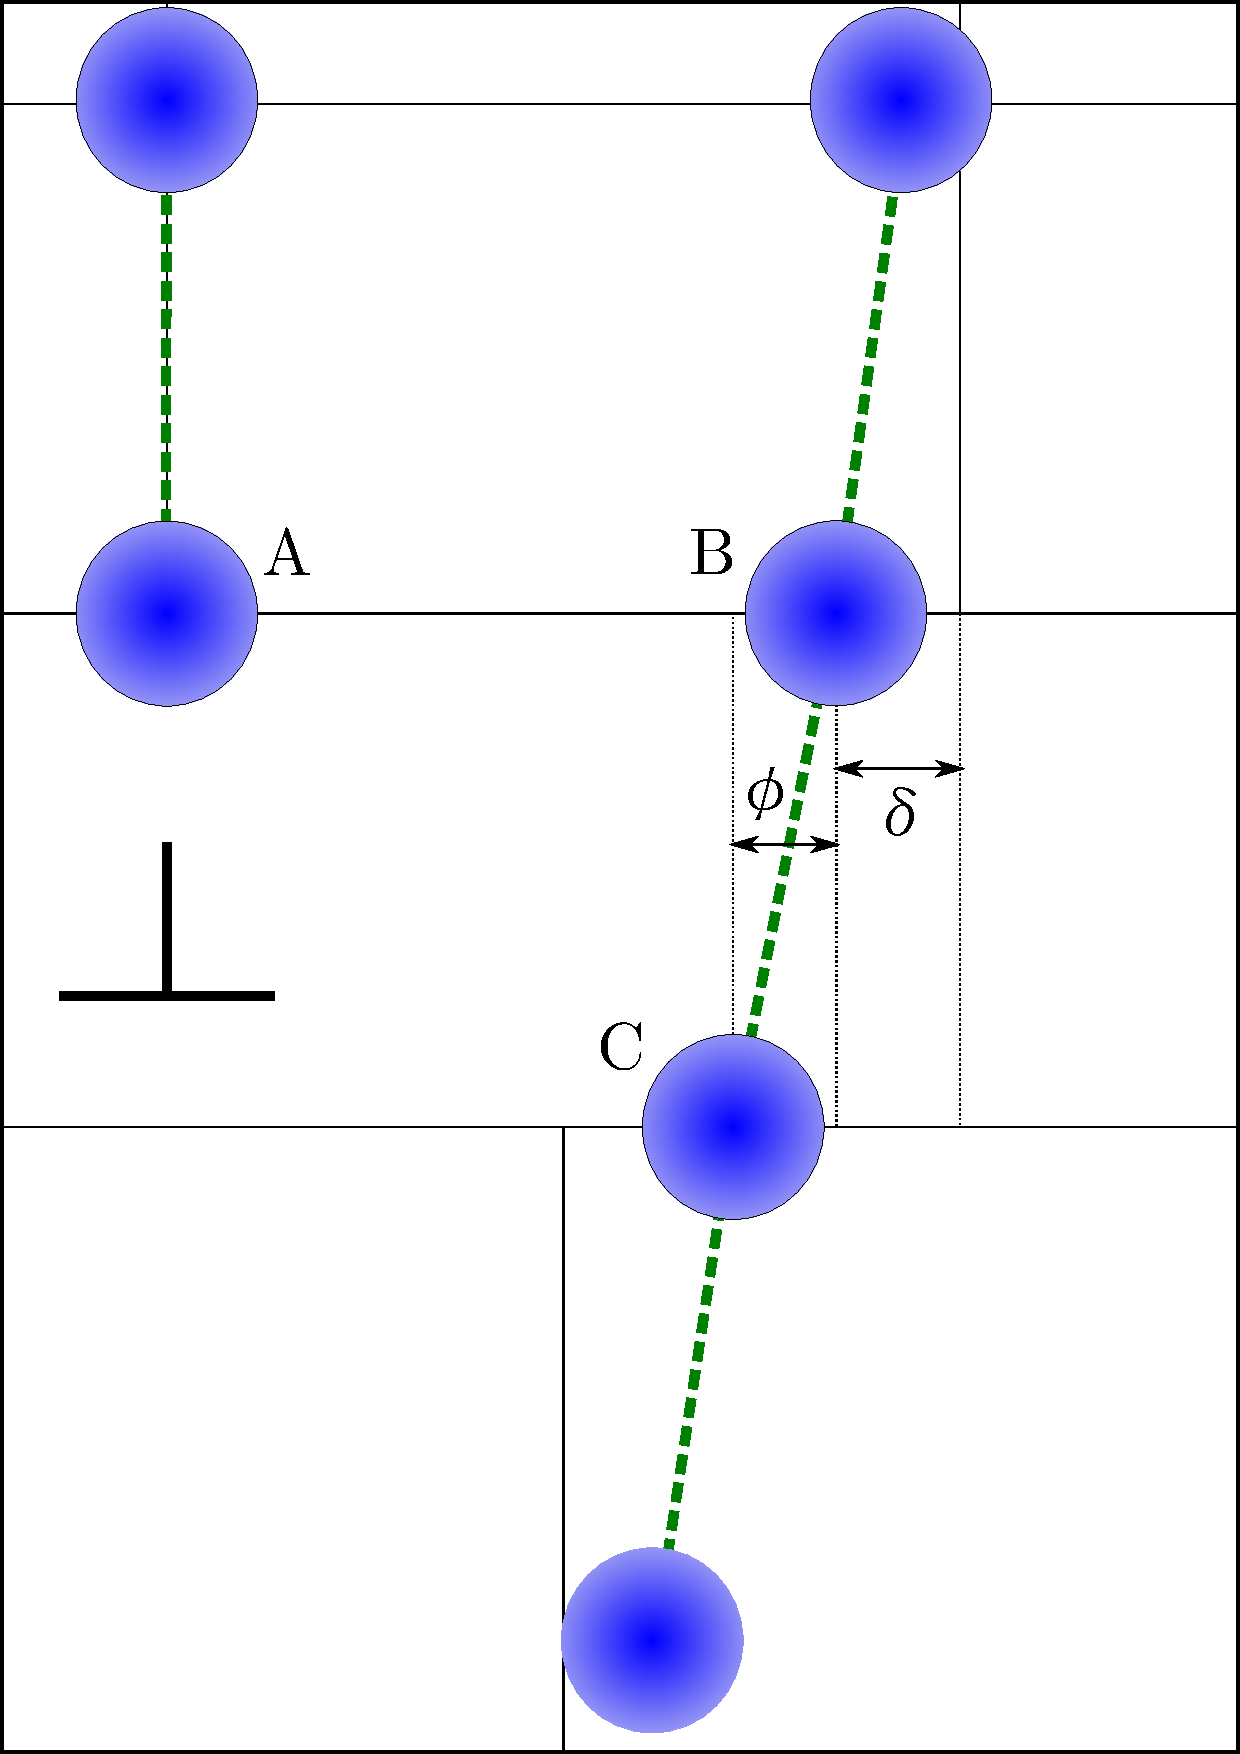
\includegraphics[width=0.6\textwidth]{peierls_model_detail}
\captionsetup{width=0.7\textwidth}
\caption[Local displacements around an edge dislocation.]{Detail of the local displacements around the dislocation core. $\delta$ is the extension of the bond parallel to the slip plane between atoms A and B, while $\phi$ is the misalignment of the bond across the slip plane between B and C.\label{fig:detail_of_peierls}}
\end{figure}

Atomic configurations that form a dislocation are generated by by applying a displacement field to the atoms immediately above and below the slip plane, $u(x)$ and $u'(x)$ respectively. The Peierls model then estimates the energy of the configuration by considering two restoring forces generated by the atomic arrangement. The detail is show in \autoref{fig:detail_of_peierls}. Firstly the bonds parallel the slip plane will be either extended or compressed, for example the bond between atom $A$ and $B$ has been compressed by the amount $\delta$, this will tend to oppose the concentration of misalignments to the core and is zero in the case of no displacements from the initial positions. Secondly bonds across the slip plane are misaligned, e.g. the bond between atom $B$ and $C$ is misaligned by a lateral distance of $\phi$. This misalignment energy will tend to favour the concentration of the misalignments to the core and is a maximum in the case of no displacement from the initial position.

Peierls made the assumption that the displacements vary slowly with position, i.e. that the dislocation is very wide. This means that the strain in the slip plane (e.g. bonds like $\overrightarrow{AB}$ in \autoref{fig:detail_of_peierls}) experience only small strains. The energy associated with these \emph{in-plane} strains are then described  by the application of the displacement field to the surface of two semi infinite elastic continua. 
The \emph{misalignment} energy of bonds across the slip plane (bonds like $\overrightarrow{BC}$ in \autoref{fig:detail_of_peierls}) is assumed to be a periodic function, specifically a simple sinusoidal variation is taken to be the form of the misalignment potential:

\begin{equation}
U_{mis} = C \sin \left(\frac{2\pi \phi}{d} \right) \label{eqn:Frenkel_approx}
\end{equation}
where $d$ is the slip plane spacing, and $\phi$ is the disregistry or misalignment across the slip plane.












%%%%%%%%%%%%%%%%%%%%%%%%%%%%%%%%%%%%%%%%%%%%%%%%%%%%%%%%%%%%%%%%%%%%%%%%%%%%%%%%%%%%%%


%
%
%
%
%   Sort out this Frenkel stuff
%
%
%
%
%
%


%%%%%%%%%%%%%%%%%%%%%%%%%%%%%%%%%%%%%%%%%%%%%%%%%%%%%%%%%%%%%%%%%%%%%%%%%%%%%%%%%%%%%%



The constant, $C$, has to be chosen appropriately but can be found by assuming linear elasticity holds at small strains. \citet{Frenkel1926} derived a similar sinusoidal function for the stress to form a stacking fault:










\begin{equation}
\tau_{fault} = \tau_{\text{theory}} \sin \left( \frac{2\pi \phi}{b} \right)
\end{equation}
where $b$ is the Burgers vector and $\phi$ is the misalignment across the slip plane.

The energy of the dislocation is the sum of all these contributions. There will be a configuration that is a minimum in the total energy where the in-plane forces widening the dislocation balance the misalignment forces that drive it to be narrower. This gives rise to a size, or width, of a dislocation. The width of the dislocation is defined as the distance from the core where the misalignment across the slip plane reaches half its maximum value. Peierls calculated this for an isotropic elastic solid, only accounting the atomic planes immediately adjacent to the slip plane and found it to be 

\begin{equation}
w = \frac{d}{1-\nu}
\label{eqn:width_isotropic}
\end{equation}
where $d$ is the plane spacing across the slip plane and $\nu$ is the Poisson ratio.

The stress required to move a dislocation can be calculated from the maximum energy gradient as the dislocation is displaced. Since the in-plane strains have a continuous definition in this model the displacement of the dislocation has no effect and the in-plane strain energy does not change. The energy changes therefore depend only on the misalignment energy of bonds across the slip plane and the energy of all the atoms away from the slip plane re neglected.

Peierls gave the critical stress, now known as the \emph{Peierls stress}, for an isotropic elastic material in terms of the ideal shear strength as calculated for uniform slip and accounting for only the interactions between the first plane either side of the slip plane, as
\begin{equation}
\frac{\tau_p}{\tau_{ideal}} = \frac{4 \pi}{1 - \nu} (5.8 - \log|1-\nu|\,) \exp\left(-\frac{4\pi}{1 - \nu}\right).
\end{equation}
This was refined by \citet{Nabarro1947} and the direct summation of the discrete contributions was developed by Cottrell and Nabarro \cite{Cottrell1953}. The result of that summation is
\begin{equation}
\tau_p = \frac{2\mu}{1-\nu} \exp\left( - \frac{4\pi w}{b} \right)
\end{equation}
where $\mu$ is the shear modulus and $b$ is the burgers vector and $\nu$ is the Poisson ratio. For an isotropic material the width can be substituted from \autoref{eqn:width_isotropic}:
\begin{equation}
\tau_p = \frac{2\mu}{1-\nu} \exp\left( - \frac{2\pi d}{(1-\nu)b} \right).
\end{equation}

Although this simple model made some significant assumptions the method moved dislocation theory on in two ways: firstly continuum elasticity could not account for energy changes as the dislocation moves since in an isotropic homogeneous continuum one dislocation position is identical to all others and thus there will be no energy changes as the dislocation move. Secondly this approach removes the singularity at the core predicted by continuum elasticity for Volterra dislocations.


An important point here is that the Peierls stress is extremely sensitive to the size of the dislocation, $w$, and therefore to the factors that control the width; which in turn is defined by the lattice geometry, $d/b$, and the elastic properties.



Peierls found the perhaps surprising result that the energy changes have a periodicity of $b/2$ rather than $b$, this has been ascribed to the summation procedure of the energy of the misaligned bonds across the slip plane, of which there has been much discussion \cite{Hirth_Lothe1982lattice_periodicity,Lu2000peierls}. Peierls summed over the atoms above the slip plane and below the slip plane independently, the ``double-counting'' scheme. Later models used a ``single-counting' scheme in which the assumption of small displacements is dropped and the misalignment of an atom above the slip plane is dependent on the final position of the atoms below the slip plane. This is given as the reason the Peierls barrier had a period of $b/2$ rather than $b$ \cite{Hirth_Lothe1982lattice_periodicity,Lu2000peierls} though it has been suggested that the problem is an artefact that arises from an assumption of small displacements and that using the final rather than initial positions of the atomic rows resolves the difficulties \cite{Huntington1955}. 

There is another explanation for the change in period based on symmetry arguments. The period will depend on the exact formulation of the energy and whether the $\alpha=1/2$ position is symmetrically equivalent to the $\alpha = 0$ or $ \alpha = 1$ positions. The periodicity of $b/2$ is easily explained on this basis.

Peierls assumed that both the elastic energy and the dislocation geometry remained constant as the dislocation moved and the only changes in the energy were therefore based on misaligned bonds across the slip plane. Another assumption that Peierls made was that the displacements of the atoms from the initial positions were small and so used the initial positions of the atoms in undistorted planes. These assumptions produce an atomic configuration at $\alpha=1/2$ that is the a reflection  of the $\alpha=0$ configuration across the slip plane, as shown in \autoref{fig:symmetrical_positions}. This must give the same energy for both configurations since the misalignment potential used by Peierls is  also symmetrical about this plane, i.e. the bonds are mirrored but otherwise unchanged and so cannot have changed in energy.

\begin{figure}
\centering
\begin{subfigure}{0.5\textwidth}
\centering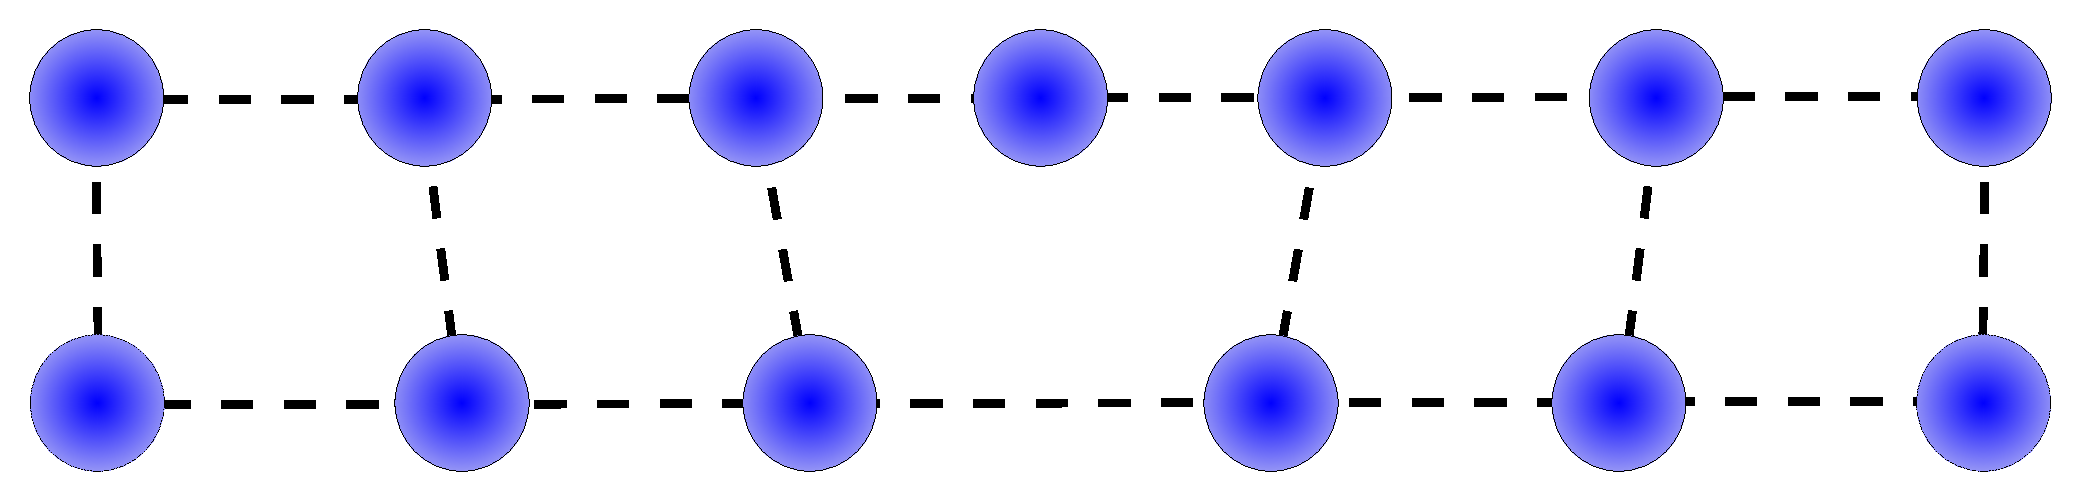
\includegraphics[width=\textwidth]{Edge_Dislocation_slip_plane}
\caption{The dislocation configuration for $\alpha=0$.}
\end{subfigure}


\begin{subfigure}{0.5\textwidth}
\centering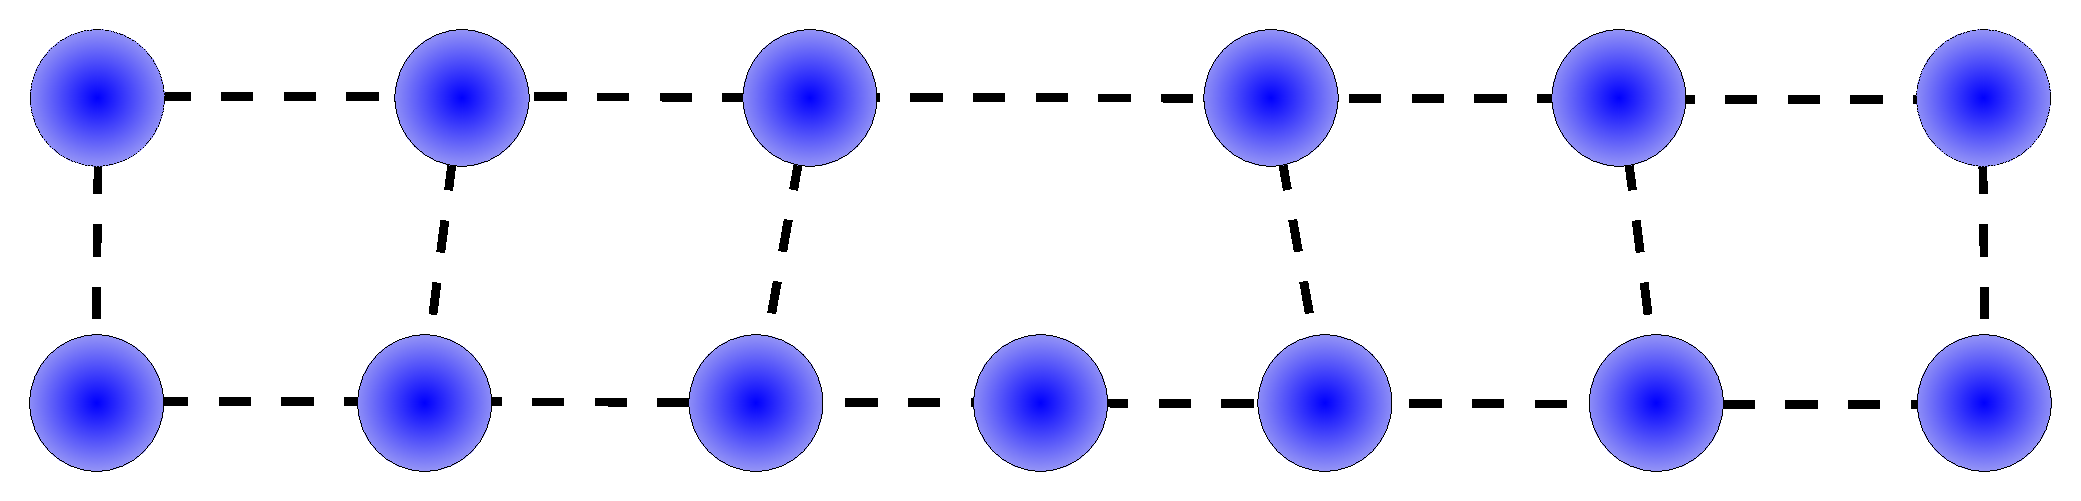
\includegraphics[width=\textwidth]{Edge_Dislocation_slip_plane_half_way}
\caption{The dislocation configuration for $\alpha=0.5$.}
\end{subfigure}

\caption[The symmetrical positions of the dislocation.]{The symmetrical positions of the dislocation. If the displacements normal to the slip plane are neglected and the model is sufficiently wide to ignore edge effects then these situations are equivalent. \citet{Peierls1940} assumed the displacements were small and that the strain energy remained constant, effectively neglecting normal displacements. \citet{Clegg2006} constrained the model to only displace atoms parallel to the slip plane, achieving the same effect.\label{fig:symmetrical_positions}}
\end{figure}


There have been many criticisms of and modifications to the Peierls model in the years since but these have largely focused on adjusting the assumptions of the original method.
In 1951 \citet{Foreman1951} introduced phenomenological potentials to describe the energy of the misaligned interactions across the slip plane, they found the width of the dislocation was predicted to be larger than that of the original treatment and was coupled with a decrease in the Peierls stress.

In 1955 \citet{Huntington1955} modified the model to double the periodicity and so account for crystals in which a displacement of half a burgers vector is not symmetrical with no displacement, or in other words broke the mirror symmetry of the slip plane. 
\citet{Maradudin1959} considered a completely atomistic three dimensional model of a screw dislocation but did not consider radial displacements. That work only evaluated the energies of the symmetric and anti-symmetric configurations and so only estimated the energy change, not the maximum stress.



In 1994 a fully discrete model was developed by \citet{Ohsawa1994}. This model made similar assumption to the original Peierls model in that the only energy changes were in the sheared misaligned bonds across the slip plane but instead of solving for an analytical solution Ohsawa et al. used numerical methods to optimise the configuration of 84 atoms,  either side of the dislocation core. The model made no assumptions about the displacement field and instead iteratively improved all the atomic positions to find the equilibrium configuration. This was done for increasing applied external stresses until there was no stable configuration, at which point slip would occur.

% Is there a term for the forces vs energy approaches to the problem?



The generalised stacking fault (GSF) energy or $\gamma$-surface was incorporated into the Peierls model by \citet{Vitek1992} and this was extended by \citet{Bulatov1997}. This improves upon an approximation in the original Peierls formulation that used the sinusoidal potential to calculate the misalignment energy. \citet{Ohsawa1994} had already attempted to address this by using alternative potentials, but used essentially arbitrary functions that fitted the shear modulus at small strains, so did not improve upon the sinusoidal form used by Peierls and Frenkel \cite{Peierls1940,Frenkel1926}. 

Bulatov et al. retained the variational approach but used density functional theory (DFT) calculations to generate a misalignment potential. They extended the model to include a three dimensional potential, allowing both lateral and vertical displacements of the atoms in the slip plane. This is important around the core where large strains mean that the energy contributions can be inaccurate. By using DFT to calculate the misalignment potential the Peierls model can bridge the length scales between the atomistic core and linear elastic far field. This is no longer analytically solvable but is not difficult to solve numerically, the only limit being computational time.

Analytical approaches have continued, \citet{Joos1997} developed a closed form solution that is valid for narrow dislocations, whereas the original model relied on the assumption of a wide dislocation for simplicity, and achieved a significantly better agreement with experiment than the original formulation. The model proposed by Jo\'{o}s and Duesbery required input parameters calculated by empirical or ab initio methods but used these as parameters of a closed form solution, in particular they required the maximum restoring stress for the glide plane, i.e. the maximum gradient of the GSF energy.

\begin{figure}
\centering
\begin{subfigure}{0.4\textwidth}
\centering
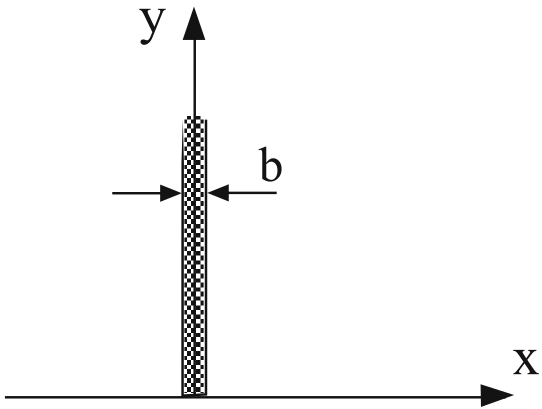
\includegraphics[width=0.75\linewidth]{Dislocation_with_discontinuity}
\caption{Volterra dislocation.\label{fig:disloc_discontinuity}}
\end{subfigure}%
\begin{subfigure}{0.4\textwidth}
\centering
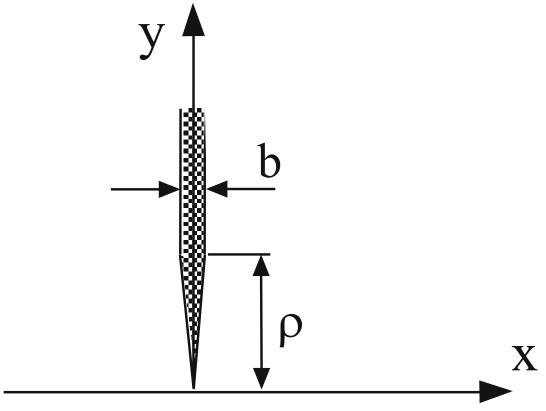
\includegraphics[width=0.75\linewidth]{Dislocation_without_discontinuity}
\caption{Lubarda dislocation\label{fig:disloc_no_discontinuity}}
\end{subfigure}
\captionsetup{width=0.8\textwidth}
\caption[Volterra and Lubarda dislocations.]{The displacement discontinuities in the traditional Volterra dislocation and that used by Lubarda and Markenscoff that removes the singularity at the core. From \cite{Lubarda2007}.\label{fig:discontinuity}}
\end{figure}

A continuum elasticity solution was presented by \citet{Lubarda2007} which removed some of the limiting assumptions of the original Peierls model; notably the assumption of fixed dislocation geometry as the dislocation was translated from one symmetrical position to the next and that only the misfit energy of the slip plane changes as the dislocation moves and that the elastic energy away from the slip plane remains constant. The main challenge to using continuum elasticity to solve the Peierls model directly is the singularity in stress and strain at the dislocation core. 


This singularity arises where the displacement discontinuity of a Volterra dislocation across the half plane of an edge dislocation terminates at the core, as shown in \autoref{fig:disloc_discontinuity}. 


By introducing a gradual increase in the displacement discontinuity across the plane of an edge dislocation from zero at the core to $b$ at some finite distance, as shown in \ref{fig:disloc_no_discontinuity}, Lubarda and Markenscoff were able to formulate a tractable linear elastic continuum problem which was in much better agreement than previous analytical solutions. They found this distance to be be interpretable as the width of the dislocation giving rise to displacements that are consistent with the original Peierls model. 



In 2006 \citet{Clegg2006} used an atomistic approach to estimate the strains outside of the slip plane in addition to the energy of the misalignment across the slip plane. The atomic displacements were taken to have the same form as Peierls had derived, that is

\begin{equation}
u(x_0) = \pm \tan^{-1}\frac{x_0}{w}.
\end{equation}

where $x_0$ is the initial coordinate in the dimension parallel to the burgers vector and $w$ is the dislocation width, now a parameter to be optimised with no closed form solution. The misalignment energy was taken to be sinusoidal by analogy with \citet{Frenkel1926}
\begin{equation}
U^{\text{x}} = \frac{Gb^3}{4\pi^2 d} \sum_n \left[ 1 - \cos \left(\frac{2\pi \phi_n}{b} \right)\right] \label{eqn:frenkel_approx}
\end{equation}
where $G$ is the shear modulus, $b$ is the Burgers vector, $d$ is the slip plane spacing, and $\phi$ is the misalignment in units of distance, as shown in \autoref{fig:detail_of_peierls}.



This arises from the requirement that Hooke's law be obeyed at small displacements and that the energy be periodic over a distance $b$. A schematic of the displacement and dimensions is shown in \autoref{fig:schematic_misalignment}.
The strain is approximately given by 
\begin{equation}
\gamma_{\text{xy}} = \frac{\phi}{d}
\end{equation}
and so the stored elastic energy is 
\begin{align}
U_{\text{elastic}} = \frac{1}{2} G \gamma_{\text{xy}}^2 V \nonumber\\
U_{\text{elastic}} = \frac{G}{2} \frac{\phi^2}{d^2} b d l \label{eqn:strain_energy}
\end{align}
where $l$ is the length of the unit cell or element into the plane of the diagram in \autoref{fig:schematic_misalignment}

For small values of $\phi$ we can use the Taylor expansion of the cosine,
\begin{equation}
\cos(x) = 1 - \frac{x^2}{2} + \frac{x^4}{24} - \dots
\end{equation}
and rewrite \autoref{eqn:frenkel_approx} for a single unit cell or element as
\begin{equation}
U^{\text{x}} = \frac{Gb^3}{4\pi^2 d} \frac{2 \pi^2 \phi^2}{b^2}
\end{equation}
which simplifies to 
\begin{equation}
U^{\text{x}} = \frac{G}{2} \frac{\phi^2}{d^2} b d
\end{equation}
which is a line energy in units of \si{\joule\per\meter} so as an absolute energy is
\begin{equation}
U^{\text{x}} = \frac{G}{2} \frac{\phi^2}{d^2} b d l
\end{equation}
which is the same as \autoref{eqn:strain_energy}.









\begin{figure}
\centering
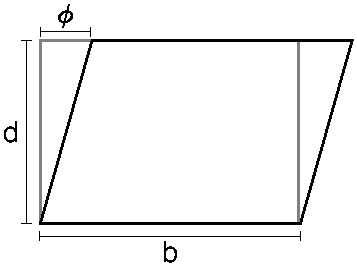
\includegraphics[]{Misalignment_of_an_element}
\captionsetup{width=0.5\textwidth}
\caption[Schematic of a misaligned unit cell]{Schematic of the misalignment of a unit cell as might be expected at the slip plane. The quantities $b$ and $d$ are the equilibrium lengths in the unstrained state, $\phi$ is the lateral displacement. \label{fig:schematic_misalignment}}
\end{figure}

The in-plane strain energy was taken to be 
\begin{equation}
U^{\text{i}} = \frac{E}{2(1-\nu^2)} (b\cdot d) \sum_n \epsilon_n^2
\end{equation}

where $E$ is the Young's modulus, $\nu$ is the Poisson ratio, $b$ is the Burgers vector, $d$ is the slip plane spacing, $\epsilon$ is the strain calculated by $\epsilon = \delta/b$, and $\delta$ is the extension of an in plane bond, as shown in \autoref{fig:detail_of_peierls}. The energies are then summed over interaction between atomic rows extending 1000 atomic spacings either side of the dislocation core.

The width no longer has an analytical solution so must be found numerically, it is generally assumed that the true value is the value that gives the lowest energy of the dislocation. The variation of the energy was shown to be smooth and have only one minimum because the misalignment energy is monotonically increasing with increasing width and the elastic in plane strain energy is monotonically decreasing.

It is interesting to note that this formulation restores the symmetry that is destroyed in the calculation of elastic energy by continuum elasticity. The strains above and below the slip plane are symmetric, so despite allowing the strain energy to vary as the dislocation moves this model has the same period as the original Peierls model of $b/2$.










































